\documentclass[letterpaper]{article}

\usepackage{longtable}
\usepackage{booktabs}
\usepackage{graphicx}
\usepackage{float}
\usepackage{hyperref}


\title{Venus Verification Results for VNN-COMP 2020}

\author{Elena Botoeva, Panagiotis Kouvaros, Jan Kronqvist, \\ Alessio
Lomuscio and Ruth Misener \\ Department of Computing, Imperial College
London, UK}
\begin{document}

\maketitle

\section{Introduction}

This document reports Venus's verification results for  the ACASXU and
PAT-FCN benchmarks of VNN-COMP 2020.

Venus~\cite{Botoeva+20} is a complete verification toolkit for
Relu-based feed-forward neural networks. It can be used to check
reachability and local adversarial robustness properties. Venus
implements a MILP-based verification method whereby it leverages
dependency relations between the ReLU nodes to reduce the search space
that needs to be considered during branch-and-bound. It additionally
implements methods based on symbolic interval propagation and input
domain splitting.

Venus participated in the PWL category. The experiments were carried
out on an Intel   Core i7-7700K  (4  cores)  equipped  with  16GB
RAM,  running Linux kernel 4.15. The code of Venus is available at
\url{https://vas.doc.ic.ac.uk/software/neural/}.

\section{Results}

\subsection{ACASXU-ALL}

\begin{figure}[H]
	\centering
	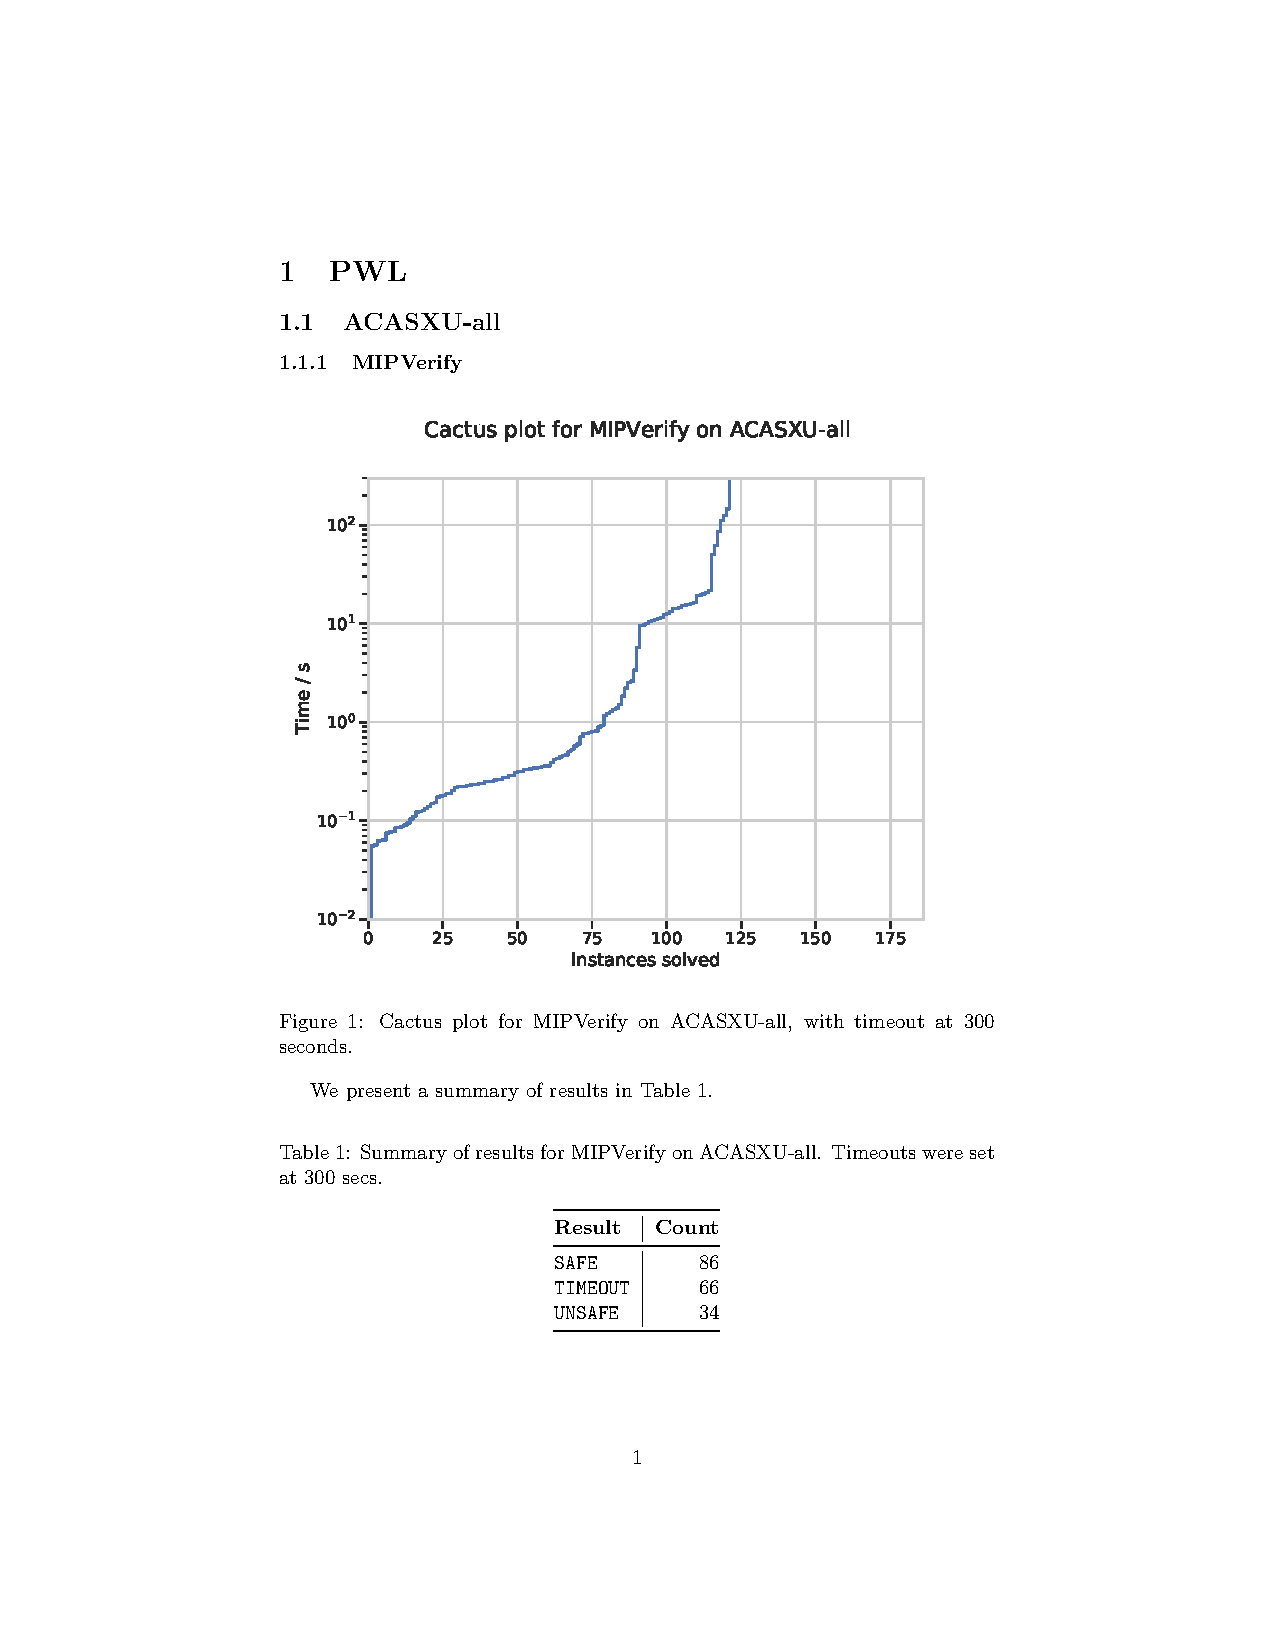
\includegraphics[width=0.8\textwidth]{evaluation/latex/acasxu-all.pdf}
	\caption{ACASXU-ALL Cactus Plot}
\end{figure}

\documentclass{article}%
\usepackage[T1]{fontenc}%
\usepackage[utf8]{inputenc}%
\usepackage{lmodern}%
\usepackage{textcomp}%
\usepackage{lastpage}%
\usepackage{graphicx}%
\usepackage{longtable}%
\usepackage{booktabs}%
%
%
%
\begin{document}%
\normalsize%
\section{PWL}%
\label{sec:PWL}%
\subsection{ACASXU{-}all}%
\label{subsec:ACASXU{-}all}%
\subsubsection{MIPVerify}%
\label{ssubsec:MIPVerify}%


\begin{figure}[htb]%
\centering%
\includegraphics[width=\textwidth]{/tmp/pylatex-tmp.b9yz5ggk/e0167153-e123-4a3c-9ded-08ac68469fb6.pdf}%
\caption{Cactus plot for MIPVerify on ACASXU{-}all, with timeout at 300 seconds.}%
\end{figure}

%
We present a summary of results in Table %
\ref{tab:mipverify/ACASXU{-}all{-}summary}%
.%


\begin{table}[!h]%
\caption{Summary of results for MIPVerify on ACASXU{-}all. Timeouts were set at 300 secs.}%
\label{tab:mipverify/ACASXU{-}all{-}summary}%
\begin{longtable}{@{}l|r@{}}%
\toprule%
\textbf{Result}&\textbf{Count}\\%
\midrule%
\verb|SAFE|&86\\%
\verb|TIMEOUT|&66\\%
\verb|UNSAFE|&34\\\bottomrule%
%
\end{longtable}%
\end{table}

%
\begin{longtable}{@{}cll|r@{}}%
\toprule%
\textbf{Prop}&\textbf{Net}&\textbf{Result}&\textbf{Runtime / s}\\%
\midrule%
\endhead%
1&1{-}1&—&—\\%
1&1{-}2&—&—\\%
1&1{-}3&—&—\\%
1&1{-}4&—&—\\%
1&1{-}5&—&—\\%
1&1{-}6&—&—\\%
1&1{-}7&—&—\\%
1&1{-}8&\verb|SAFE|&62.35\\%
1&1{-}9&\verb|SAFE|&86.62\\%
1&2{-}1&—&—\\%
1&2{-}2&—&—\\%
1&2{-}3&—&—\\%
1&2{-}4&—&—\\%
1&2{-}5&—&—\\%
1&2{-}6&—&—\\%
1&2{-}7&—&—\\%
1&2{-}8&—&—\\%
1&2{-}9&—&—\\%
1&3{-}1&—&—\\%
1&3{-}2&—&—\\%
1&3{-}3&—&—\\%
1&3{-}4&—&—\\%
1&3{-}5&—&—\\%
1&3{-}6&—&—\\%
1&3{-}7&—&—\\%
1&3{-}8&—&—\\%
1&3{-}9&—&—\\%
1&4{-}1&—&—\\%
1&4{-}2&—&—\\%
1&4{-}3&—&—\\%
1&4{-}4&—&—\\%
1&4{-}5&—&—\\%
1&4{-}6&—&—\\%
1&4{-}7&—&—\\%
1&4{-}8&—&—\\%
1&4{-}9&—&—\\%
1&5{-}1&—&—\\%
1&5{-}2&—&—\\%
1&5{-}3&—&—\\%
1&5{-}4&—&—\\%
1&5{-}5&—&—\\%
1&5{-}6&—&—\\%
1&5{-}7&—&—\\%
1&5{-}8&—&—\\%
1&5{-}9&—&—\\%
2&1{-}1&—&—\\%
2&1{-}2&—&—\\%
2&1{-}3&—&—\\%
2&1{-}4&—&—\\%
2&1{-}5&—&—\\%
2&1{-}6&\verb|UNSAFE|&125.49\\%
2&1{-}7&—&—\\%
2&1{-}8&—&—\\%
2&1{-}9&—&—\\%
2&2{-}1&\verb|UNSAFE|&21.86\\%
2&2{-}2&\verb|UNSAFE|&145.67\\%
2&2{-}3&\verb|UNSAFE|&10.00\\%
2&2{-}4&\verb|UNSAFE|&20.02\\%
2&2{-}5&\verb|UNSAFE|&11.32\\%
2&2{-}6&\verb|UNSAFE|&12.28\\%
2&2{-}7&\verb|UNSAFE|&19.51\\%
2&2{-}8&\verb|UNSAFE|&15.44\\%
2&2{-}9&—&—\\%
2&3{-}1&\verb|UNSAFE|&9.59\\%
2&3{-}2&—&—\\%
2&3{-}3&—&—\\%
2&3{-}4&\verb|UNSAFE|&9.71\\%
2&3{-}5&\verb|UNSAFE|&12.69\\%
2&3{-}6&—&—\\%
2&3{-}7&—&—\\%
2&3{-}8&\verb|UNSAFE|&110.51\\%
2&3{-}9&\verb|UNSAFE|&14.67\\%
2&4{-}1&—&—\\%
2&4{-}2&—&—\\%
2&4{-}3&\verb|UNSAFE|&11.07\\%
2&4{-}4&—&—\\%
2&4{-}5&\verb|UNSAFE|&14.34\\%
2&4{-}6&\verb|UNSAFE|&14.35\\%
2&4{-}7&\verb|UNSAFE|&11.48\\%
2&4{-}8&\verb|UNSAFE|&15.68\\%
2&4{-}9&\verb|UNSAFE|&50.52\\%
2&5{-}1&\verb|UNSAFE|&13.18\\%
2&5{-}2&\verb|UNSAFE|&10.78\\%
2&5{-}3&—&—\\%
2&5{-}4&\verb|UNSAFE|&10.57\\%
2&5{-}5&\verb|UNSAFE|&16.04\\%
2&5{-}6&\verb|UNSAFE|&15.22\\%
2&5{-}7&\verb|UNSAFE|&16.50\\%
2&5{-}8&\verb|UNSAFE|&20.79\\%
2&5{-}9&\verb|UNSAFE|&19.19\\%
3&1{-}1&\verb|SAFE|&3.38\\%
3&1{-}2&\verb|SAFE|&1.22\\%
3&1{-}3&\verb|SAFE|&5.72\\%
3&1{-}4&\verb|SAFE|&0.32\\%
3&1{-}5&\verb|SAFE|&0.22\\%
3&1{-}6&\verb|SAFE|&0.12\\%
3&1{-}7&\verb|UNSAFE|&0.09\\%
3&1{-}8&\verb|UNSAFE|&0.08\\%
3&1{-}9&\verb|UNSAFE|&0.06\\%
3&2{-}1&\verb|SAFE|&0.89\\%
3&2{-}2&\verb|SAFE|&0.81\\%
3&2{-}3&\verb|SAFE|&2.23\\%
3&2{-}4&\verb|SAFE|&0.08\\%
3&2{-}5&\verb|SAFE|&0.24\\%
3&2{-}6&\verb|SAFE|&0.13\\%
3&2{-}7&\verb|SAFE|&0.18\\%
3&2{-}8&\verb|SAFE|&0.09\\%
3&2{-}9&\verb|SAFE|&0.06\\%
3&3{-}1&\verb|SAFE|&0.22\\%
3&3{-}2&\verb|SAFE|&2.54\\%
3&3{-}3&\verb|SAFE|&0.50\\%
3&3{-}4&\verb|SAFE|&1.17\\%
3&3{-}5&\verb|SAFE|&0.23\\%
3&3{-}6&\verb|SAFE|&0.77\\%
3&3{-}7&\verb|SAFE|&0.06\\%
3&3{-}8&\verb|SAFE|&0.22\\%
3&3{-}9&\verb|SAFE|&0.12\\%
3&4{-}1&\verb|SAFE|&0.57\\%
3&4{-}2&\verb|SAFE|&1.27\\%
3&4{-}3&\verb|SAFE|&1.35\\%
3&4{-}4&\verb|SAFE|&0.31\\%
3&4{-}5&\verb|SAFE|&0.10\\%
3&4{-}6&\verb|SAFE|&0.79\\%
3&4{-}7&\verb|SAFE|&0.15\\%
3&4{-}8&\verb|SAFE|&0.19\\%
3&4{-}9&\verb|SAFE|&0.29\\%
3&5{-}1&\verb|SAFE|&1.39\\%
3&5{-}2&\verb|SAFE|&0.26\\%
3&5{-}3&\verb|SAFE|&0.44\\%
3&5{-}4&\verb|SAFE|&0.22\\%
3&5{-}5&\verb|SAFE|&0.34\\%
3&5{-}6&\verb|SAFE|&0.27\\%
3&5{-}7&\verb|SAFE|&0.06\\%
3&5{-}8&\verb|SAFE|&0.20\\%
3&5{-}9&\verb|SAFE|&0.09\\%
4&1{-}1&\verb|SAFE|&0.81\\%
4&1{-}2&\verb|SAFE|&0.71\\%
4&1{-}3&\verb|SAFE|&1.52\\%
4&1{-}4&\verb|SAFE|&0.26\\%
4&1{-}5&\verb|SAFE|&0.33\\%
4&1{-}6&\verb|SAFE|&0.25\\%
4&1{-}7&\verb|UNSAFE|&0.07\\%
4&1{-}8&\verb|UNSAFE|&0.09\\%
4&1{-}9&\verb|UNSAFE|&0.06\\%
4&2{-}1&\verb|SAFE|&0.77\\%
4&2{-}2&\verb|SAFE|&0.93\\%
4&2{-}3&\verb|SAFE|&0.19\\%
4&2{-}4&\verb|SAFE|&0.25\\%
4&2{-}5&\verb|SAFE|&0.32\\%
4&2{-}6&\verb|SAFE|&0.35\\%
4&2{-}7&\verb|SAFE|&0.18\\%
4&2{-}8&\verb|SAFE|&1.84\\%
4&2{-}9&\verb|SAFE|&0.08\\%
4&3{-}1&\verb|SAFE|&0.36\\%
4&3{-}2&\verb|SAFE|&0.24\\%
4&3{-}3&\verb|SAFE|&0.14\\%
4&3{-}4&\verb|SAFE|&0.23\\%
4&3{-}5&\verb|SAFE|&0.53\\%
4&3{-}6&\verb|SAFE|&0.42\\%
4&3{-}7&\verb|SAFE|&0.15\\%
4&3{-}8&\verb|SAFE|&0.46\\%
4&3{-}9&\verb|SAFE|&0.36\\%
4&4{-}1&\verb|SAFE|&0.11\\%
4&4{-}2&\verb|SAFE|&0.46\\%
4&4{-}3&\verb|SAFE|&0.43\\%
4&4{-}4&\verb|SAFE|&2.61\\%
4&4{-}5&\verb|SAFE|&0.29\\%
4&4{-}6&\verb|SAFE|&0.34\\%
4&4{-}7&\verb|SAFE|&0.17\\%
4&4{-}8&\verb|SAFE|&0.33\\%
4&4{-}9&\verb|SAFE|&0.39\\%
4&5{-}1&\verb|SAFE|&0.34\\%
4&5{-}2&\verb|SAFE|&0.25\\%
4&5{-}3&\verb|SAFE|&0.60\\%
4&5{-}4&\verb|SAFE|&0.26\\%
4&5{-}5&\verb|SAFE|&0.28\\%
4&5{-}6&\verb|SAFE|&0.23\\%
4&5{-}7&\verb|SAFE|&0.13\\%
4&5{-}8&\verb|SAFE|&0.33\\%
4&5{-}9&\verb|SAFE|&0.23\\%
5&1{-}1&—&—\\%
6&1{-}1&—&—\\%
7&1{-}9&—&—\\%
8&2{-}9&—&—\\%
9&3{-}3&—&—\\%
10&4{-}5&—&—\\\bottomrule%
%
\end{longtable}

%
\end{document}


\subsection{ACASXU-HARD}


\documentclass{article}%
\usepackage[T1]{fontenc}%
\usepackage[utf8]{inputenc}%
\usepackage{lmodern}%
\usepackage{textcomp}%
\usepackage{lastpage}%
\usepackage{graphicx}%
\usepackage{longtable}%
\usepackage{booktabs}%
%
%
%
\begin{document}%
\normalsize%
\section{PWL}%
\label{sec:PWL}%
\subsection{ACASXU{-}hard}%
\label{subsec:ACASXU{-}hard}%
\subsubsection{MIPVerify}%
\label{ssubsec:MIPVerify}%


\begin{figure}[htb]%
\centering%
\includegraphics[width=\textwidth]{/tmp/pylatex-tmp.bm9xo0cf/9fed2472-0b7a-4028-832a-afc5326ba35a.pdf}%
\caption{Cactus plot for MIPVerify on ACASXU{-}hard, with timeout at 21600 seconds.}%
\end{figure}

%
We present a summary of results in Table %
\ref{tab:mipverify/ACASXU{-}hard{-}summary}%
.%


\begin{table}[!h]%
\caption{Summary of results for MIPVerify on ACASXU{-}hard. Timeouts were set at 21600 secs.}%
\label{tab:mipverify/ACASXU{-}hard{-}summary}%
\begin{longtable}{@{}l|r@{}}%
\toprule%
\textbf{Result}&\textbf{Count}\\%
\midrule%
\verb|TIMEOUT|&6\\%
\verb|SAFE|&2\\%
\verb|UNSAFE|&2\\\bottomrule%
%
\end{longtable}%
\end{table}

%
\begin{longtable}{@{}cll|r@{}}%
\toprule%
\textbf{Prop}&\textbf{Net}&\textbf{Result}&\textbf{Runtime / s}\\%
\midrule%
\endhead%
1&4{-}6&—&—\\%
1&4{-}8&—&—\\%
2&3{-}3&—&—\\%
2&4{-}2&—&—\\%
2&4{-}9&\verb|UNSAFE|&37.42\\%
2&5{-}3&\verb|UNSAFE|&5390.41\\%
3&3{-}6&\verb|SAFE|&0.64\\%
3&5{-}1&\verb|SAFE|&1.30\\%
7&1{-}9&—&—\\%
9&3{-}3&—&—\\\bottomrule%
%
\end{longtable}

%
\end{document}


\subsection{PAT-FCN}

\begin{figure}[H]
	\centering
	\includegraphics[width=0.8\textwidth]{evaluation/latex/mnist.pdf}
	\caption{PAT-FCN Cactus Plot}
\end{figure}

\input{evaluation/latex/mnist.tex}

\bibliographystyle{plain}

\begin{thebibliography}{1}

\bibitem{Botoeva+20}
E.~Botoeva, P.~Kouvaros, J.~Kronqvist, A.~Lomuscio, and R.~Misener.
\newblock Efficient verification of neural networks via dependency analysis.
\newblock In {\em Proceedings of the 34th AAAI Conference on Artificial
  Intelligence (AAAI20)}. {AAAI} Press, 2020.

\end{thebibliography}

\end{document}
